\chapter{Problemløsning}\label{ch:chlabel}

INTRODUKTION
% Ret eller omformuler endelig hvis du har noget bedre
I dette kapitel stilles der krav til programmet for at løse problemet på den bedste måde. Ud fra disse krav vil der blive lavet et design til løsningen. Til sidst forklares det hvordan dette design er implementeret, og hvorden programmeringen og datastrukturen er stillet op. Der gives også beskrivelser og forklaringer af flere af funktionerne fra kildekoden. 

%det hvordan et program kan blive til en løsning, på det problem der er opstillet i problemformuleringen. Først ved at formulerer et antal konkrete krav til løsningen. Efterfølgende designes der et program ud fra disse krav. Til sidst forklares det hvordan dette design er implementeret, ved at beskrive programmeringsstil og datastruktur. Der gives også beskrivelse og forklaringer af flere funktioner fra kildekoden.

\section{Krav til løsningen}
For at lave en funktionel løsning til projektets problemformulering, er det nødvendigt at opstille en række krav. Disse krav skaber et overblik over hvilke opgaver løsningen skal være i stand til at fuldføre.
\\
Et af de grundlæggende krav til løsningen, er at den skal være i stand til at opstille et kampprogram. Dette kampprogram skal overholde reglerne for stævner i Kidzliga-floorball, som er stillet af Floorball Danmark \cite{kidzRegler}. Derfor er det nødvendigt at tage disse regler i betragtning, når et kampprogram bliver udarbejdet.\\
I dette afsnit er de relevante regler listet i rækkefølge efter prioritet. Prioriteringen bestemmer hvilke regler der er vigtigst at overholde, og hvilke der kan undlades, i tilfælde af at det ikke er muligt at implementere dem alle.
\begin{itemize}
    \item \textit{En kamp varer seks minutter,\ og der skal være en til to minutters pause mellem hver kamp.} I forbindelse med projektet er det besluttet at sætte et krav på to minutters pause mellem hver kamp, da det er mere specifikt.
    \item \textit{Alle hold der deltager skal have cirka seks kampe.} Reglerne er i dette tilfælde heller ikke specificeret yderligere. Derfor er kravet i projektet gjort mere specifikt ved at hvert hold skal have seks kampe. Kun hvis dette ikke er muligt må et eller flere hold spille en kamp mere eller mindre. 
    \item \textit{Alle kampe i en runde skal startes og afsluttes på samme tid.} Denne regel er med til at sikre, at kampprogrammet ikke skrider så meget, at et hold pludselig skal spille to steder på samme tid, eller meget kort tid efter hinanden, som beskrevet i følgende regel.
    \item \textit{Alle hold skal have mindst én hvilekamp mellem hver kamp}, hvis det er muligt. Er det ikke muligt at indlægge en hvilekamp, tilstræbes det ifølge reglerne, at holdet, der spiller flere runder i træk, spiller på samme bane. I dette projekt er det fastsat som en regel at kampen skal foregå på samme bane, i tilfælde af at en hvilekamp ikke er mulig. 
    \item \textit{Der er defineret fire forskellige niveauer i Kidzliga: N, A, B og C.} Niveauerne er delt op, så C er det højeste niveau, så kommer B, A og til sidst N, som står for nybegynder. Et hold må kun spille mod et andet hold, der er på det samme niveau.
    \item Det kan forekomme at et kampprogram bliver hængt op i en hal, hvor stævnet bliver afviklet. Derfor stilles der et krav til løsningen, om at \textit{det udviklede kampprogram skal være opstillet på en præsentabel måde.} Det bestemmes herudfra, at opdeling i runder skal fremstå tydeligt, hvor hver runde er opdelt i kampe. Her skal banenummer, niveau og startstid for hver runde også stå.
\end{itemize} 
Det er nødvendigt at overholde disse specifikke regler, da løsningen er afgrænset til Kidzliga. Kravene til løsningen er dog ikke opstillet udelukkende på baggrund af reglerne for spillet.
\\\\
Ydereligere, opstilles krav for løsningen, som ikke er direkte stillet af Floorball Danmark. Disse regler fremsættes for at øge kvaliteten af stævneplanen. Et menneske vil naturligt følge dem, men reglerne skal defineres klart, for at et program også overholder dem.
\begin{itemize}
    \item \textit{Et hold må ikke spille mere end 2 kampe i træk.} Dette er en udvidelse af reglen om at der skal være en hvilkekamp mellem hver kamp og gælder når dette ikke kan lade sig gøre. 
    \item \textit{Hvert hold skal spille mod et andet hold igen, så få gange som muligt, og to hold må ikke spille mod hinanden to kampe i træk.} Dette er besluttet for at sikre at hvert hold kommer til at spille med så mange forskellige hold som muligt.
\end{itemize}

Problemformuleringen nødvendiggør også et krav, om at stævneplanen skal være fleksibel. Det skal være muligt at foretage ændringer i stævneplanen, efter det er blevet udarbejdet. Løsningen tillader brugeren at tilføje og fjerne hold fra stævneplanen. Dette vil gøre stævneplanen mere fleksibel, da brugeren får mulighed for at lave hurtige ændringer i et allerede eksisterende kampprogram.
\\\\
%Ud fra disse krav er det muligt at designe et program, som er en fyldestgørende løsning på problemformuleringen.
Ud fra disse krav er det muligt at komme frem til en ide og et overordnet design til programmet, som skal løse problemet. 
%ved ikke om det er bedre :/

\section{Design}
%Overgang til design. INTRODUKTION.
Ud fra kravene er det muligt at designe et program til at løse problemstillingen. Designet består i den overordnede ide om hvordan programmet skal fungere og hænge sammen. Samtidigt afklare designet hvordan problemet kan deles op i flere mere overkommelige opgaver, for at gøre det nemmere at udvikle et program. 
\\\\
Der er blevet lavet tre flowchart til at beskrive programmets design. Det overordnede flowchart, som viser den grove struktur af programmet. Lav en stævneplan, som viser tanken bag hvordan programmet laver en stævneplan. Til sidst er der rediger stævneplan, som viser tanken om hvordan programmet skal kunne tilføje og fjerne hold fra en eksisterende stævneplan. Det overordnede flowchart bliver gennemgået først.

\begin{figure}[H]
  \centering
  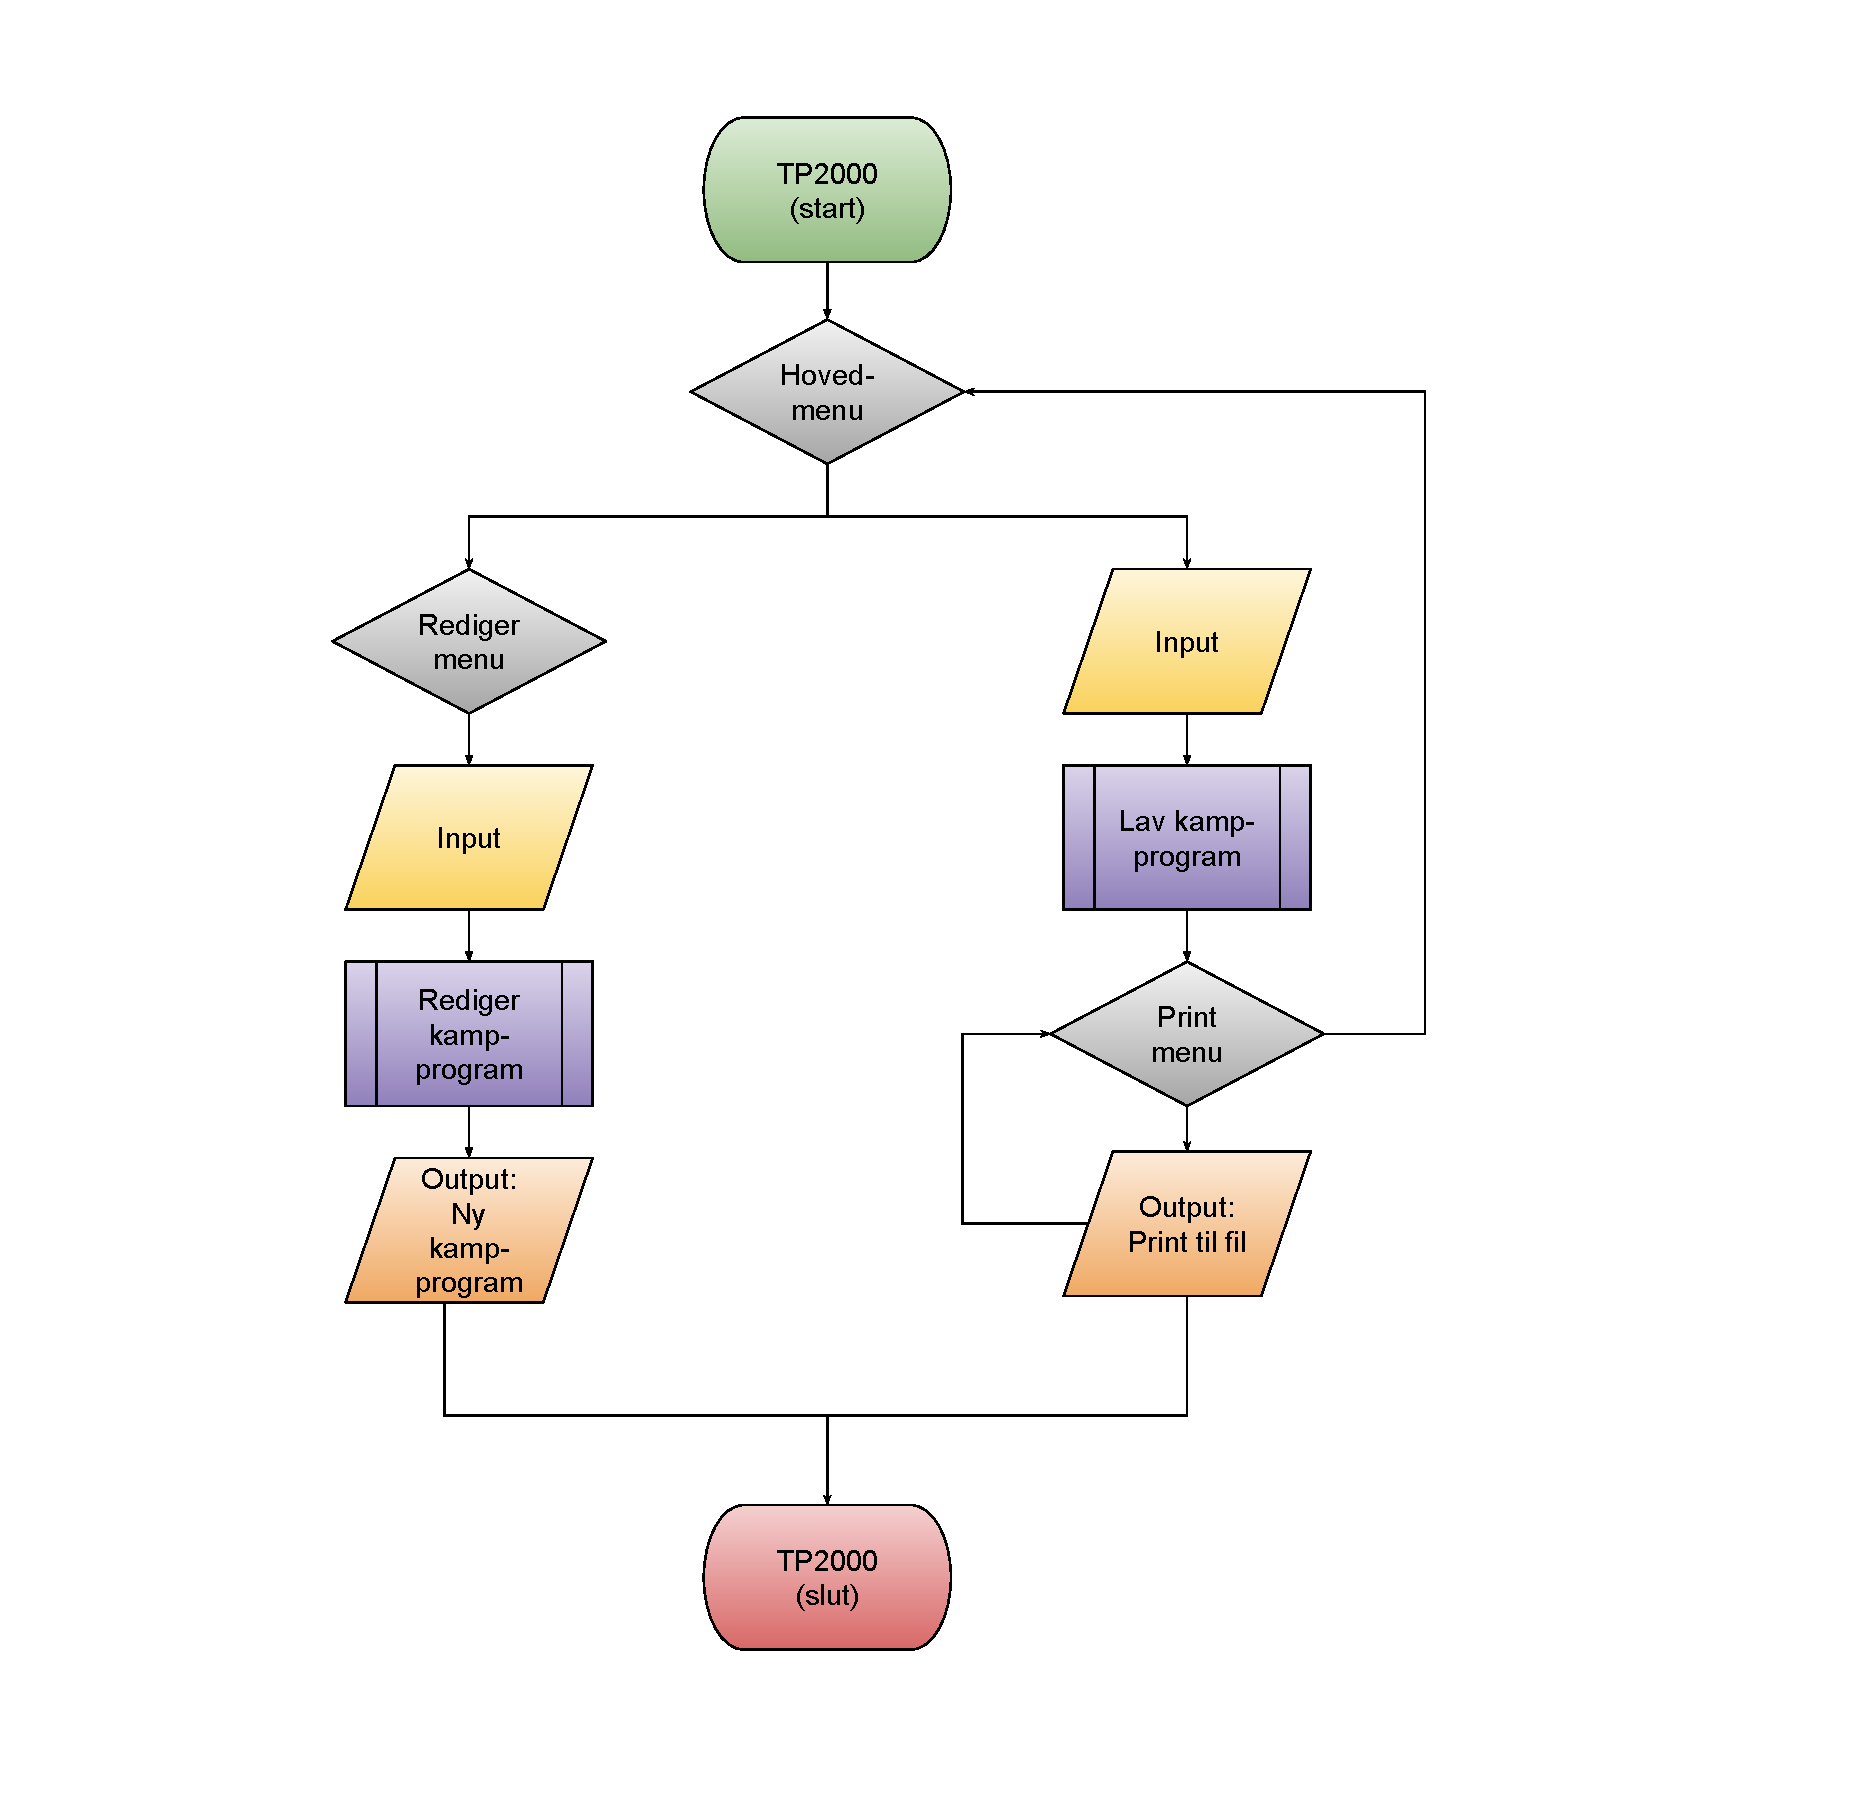
\includegraphics[width=0.9\textwidth]{figures/Overordnet.pdf}
  \caption{Flowchart over programmets overordnede struktur.}
  \label{fig:overordnet-flowchart}
\end{figure}

På figur \ref{fig:overordnet-flowchart} ses en overordnet struktur over programmets opbygning. Programmet starter med en hovedmenu, hvor brugeren skal vælge mellem to grene. Den højre gren giver mulighed for at lave en ny stævneplan, og den venstre gren giver mulighed for at redigere en allerede eksisterende stævneplan. Disse valgmuligheder er med til at give et overblik over hvad programmet kan, og giver mulighed for at brugeren selv kan bestemme hvad de ønsker at gøre med programmet.

\subsubsection{Oprettelse af stævneplan}
For at løsningen skal være i stand til at overholde de opstillede krav for oprettelse af en stævneplan, har programmet brug for disse informationer fra brugeren:
\begin{itemize}
    \item Holdnavne med niveau i en tekstfil
    \item Antal baner
    \item Starttidspunktet for stævnet
\end{itemize}
Disse informationer er nødvendige at have, for at kunne lave en stævneplan der er opstillet ordentligt og korrekt efter de andre krav og regler. 
\par
Holdnavne og niveauer indlæses fra en tekstfil, da der kan være mange hold, og man ellers kan miste overblikket, hvis input tastes gennem terminalen. Når holdnavne skrives ind på en fil bliver det mere overskueligt for brugeren. Dette kræver dog en specifik opsætning af filen, da programmet ellers ikke vil kunne læse den.
% Beskrivelse af opsætningen, 
\\\\
Kravene til opsætningen er at der skal være ét holdnavn på hver linje, efterfulgt af et komma og holdets niveau. Holdnavnet må indeholde specialtegn, men det første tegn skal være et bogstav.
Niveauet, der angives med et bogstav, må være både stort og småt.
% Eksempel
\\\\
Holdnavn1, Niveau\\
Holdnavn2, Niveau\\
...\\

Antallet af hold og starttidspunktet indlæses gennem terminalen, da disse er enklere for brugeren at taste ind.
\par
Herefter sammensættes stævneplanen. Dette sker ved brug af tilfældig sammensætning af kampe og runder, hvorefter hver runde evalueres, og der tælles fejl i forhold til hvor mange gange de vigtigste reglerne er blevet brudt. Hvis runden ingen fejl har, godkendes den, ellers bliver den sammensat anderledes indtil den er acceptabel. Hvis der ikke kan findes en rundesammensætning, som overholder de opstillede regler, startes processen forfra.\\
Der var en overvejelse om at sammensætte stævneplanen på en struktureret måde - en imitation af, hvordan et menneske ville lægge planen - og gøre det hurtigere end en person kunne gøre det. Med denne metode er der dog en risiko for at den bedste stævneplan ikke bliver fundet. Ved at bruge den tilfældige metode, bliver der sammensat flere forskellige stævneplaner tilfældigt og den bedste bliver valgt.\par
For at få det optimale resultat vil der være behov for et point-system, som giver point i forhold til de regler der ikke er givet af Floorball Danmark. Jo flere regler der bliver opfyldt jo flere point får stævneplanen. Hver stævneplan bliver hermed sammenlignet med den forrige, hvor den med flest point bliver gemt. Efter et fastsat antal iterationer, bliver den bedste printet ud.\\
Det er dog ikke det projektets program gør, da denne løsning vil tage for lang tid for programmet at komme frem til den bedste stævneplan. Dette skyldes at for at stævneplanen bliver god nok, skal programmet køres et bestemt antal gange, som er for stort i forhold til den tid det tager for programmet at komme med en god stævneplan.

\begin{figure}[H]
  \centering
  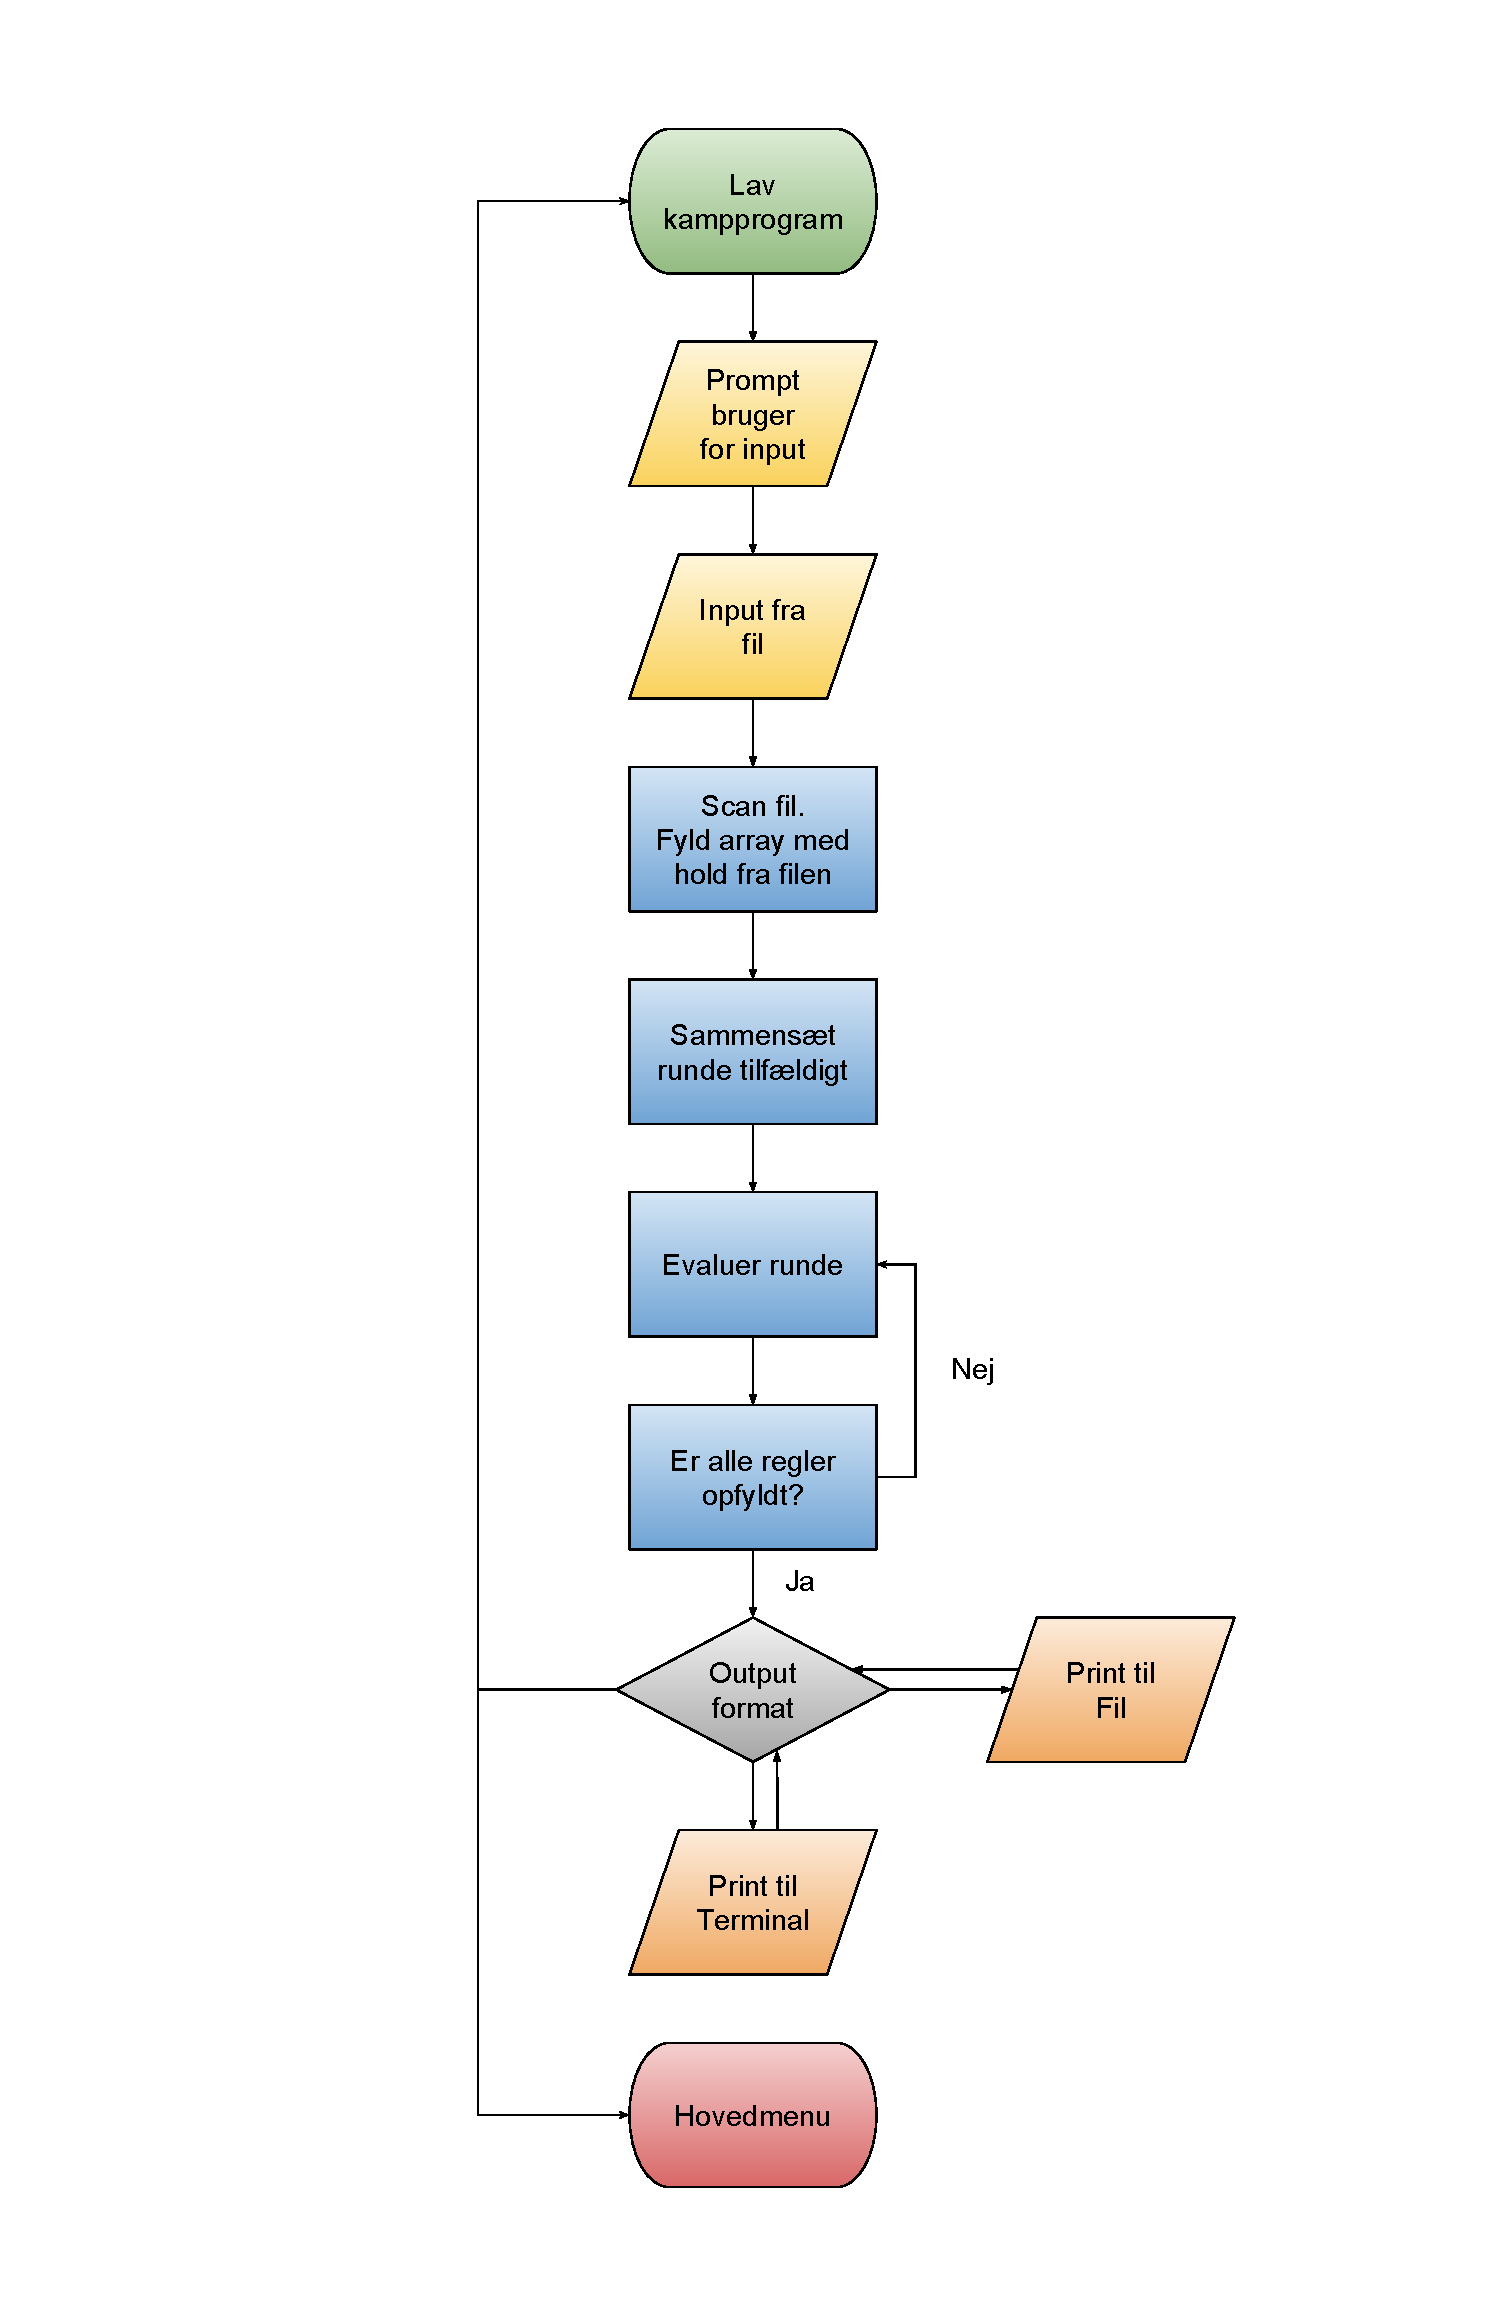
\includegraphics[width=0.7\textwidth]{figures/Lavflowchart.pdf}
  \caption{Flowchart over processen for at lave et kampprogram}
  \label{fig:lav-flowchart}
\end{figure}

Som det ses på figur \ref{fig:lav-flowchart} bliver brugeren bedt om at foretage et valg i forhold til hvilket output format der ønskes. Her er det muligt at få stævneplanen printet til terminalen, da brugeren så har mulighed for at tjekke stævneplanens sammensætning for om det ser ordentligt ud. Hvis ikke man er tilfreds kan der sammensættes en ny stævneplan. Man kan også få printet stævneplanen ud på en fil, da det er et krav, at man skal kunne printe stævneplanen ud og hænge den op i hallen.\\
Når man er færdig med at lave stævneplanen, kommer man tilbage til hovedmenuen, hvor der igen er mulighed for at vælge mellem de to grene på figur \ref{fig:overordnet-flowchart}.

\subsubsection{Redigering af stævneplan}
Hvis man vælger at redigere stævneplanen, følger man venstre gren på figur \ref{fig:overordnet-flowchart}. Som det fremstår på det overordnede flowchart, gør løsningen det muligt for en bruger at redigere en allerede eksisterende stævneplan, ved at tilføje eller fjerne hold. Dette er under betingelsen, at stævneplanen, der ønskes ændret, er af samme format som programmet bruger. 
% Indsæt rediger-kampprogram flowchart her!
\begin{figure}[H]
  \centering
  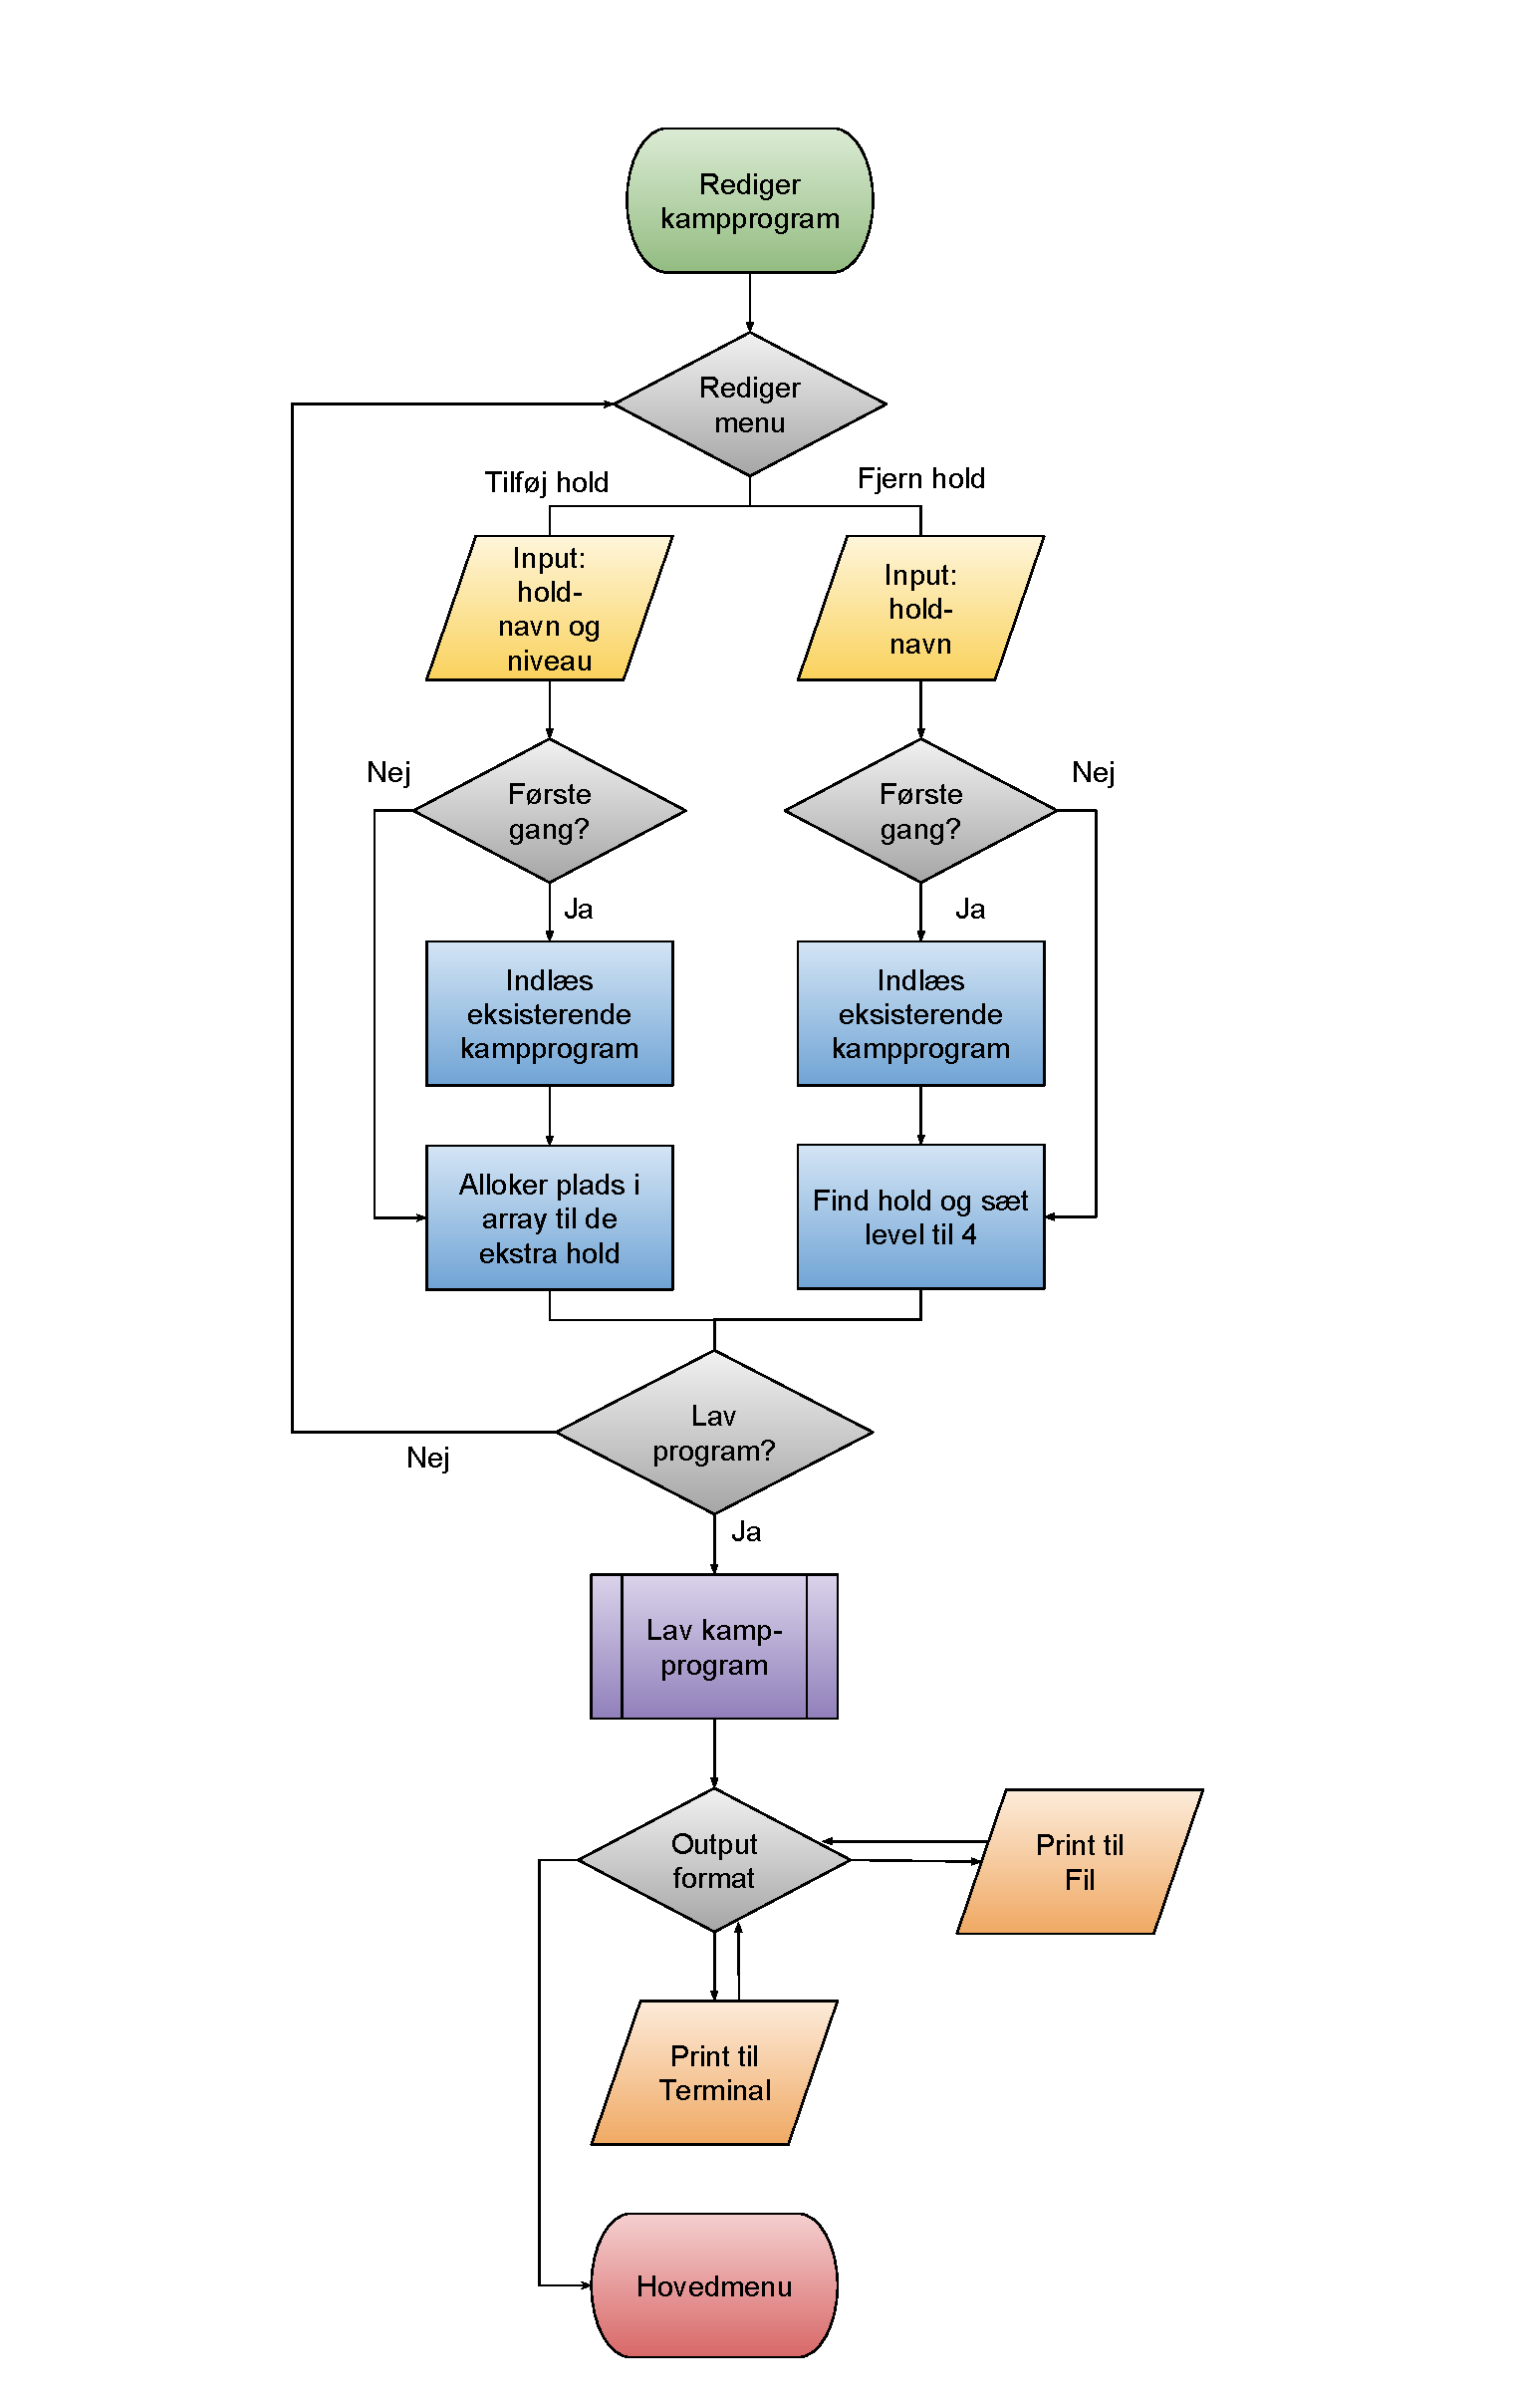
\includegraphics[width=0.7\textwidth]{figures/Redigerflowchart.pdf}
  \caption{Flowchart over processen for at redigere et kampprogram.}
  \label{fig:rediger-flowchart}
\end{figure}
% % % % % % % % % % % % % % % hest?
Måden hvorpå programmet redigerer en eksisterende stævneplan er illustreret på figur \ref{fig:rediger-flowchart}. Brugeren bedes indtaste hvilke hold der skal tilføjes eller fjernes. 
\par
Efterfølgende indlæses informationerne fra en fil med den eksisterende stævneplan, på en sådan måde, at det er muligt at arbejde med dem. Dette skal dog kun gøres én gang, inden der foretages ændringer. Efterfølgende kan der foretages flere ændringer indtil brugeren er tilfreds. Disse ændringer foretages en af gangen. 
\par
Herefter bearbejdes informationen, sådan at den stemmer overens med de ændringer brugeren ønsker. Dette kan ses i kildekode \ref{code:updateTournament} side \pageref{code:updateTournament}. Til sidst fremstilles en stævneplan med ændringerne, på samme måde som der fremstilles en ny stævneplan. Brugeren har så mulighed for at printe stævneplanen, enten i terminalen eller til en fil. I terminalen kan stævneplanen inspiceres, og der er mulighed for at lave yderligere ændringer eller generere stævneplanen igen, før det færdige kampprogram gemmes.
\par
For at gøre programmet mere fleksibelt, ville muligheden for at redigere i en stævneplan, hvor stævnet allerede er startet, være optimal. Der kan opstå situationer, hvor et hold enten er forhindret i at møde til tiden, eller er nødt til gå tidligere. Her ville muligheden for at ændre planen fra et bestemt tidspunkt gøre programmet mere fleksibelt. I dette projekt, prioriteres denne funktionalitet lavere end muligheden for at tilføje og fjerne hold, da dette vurderes til at være vigtigere.
\subsection*{Opsamling} 
Dette er ideen og designet bag programmets virkemåde og opsætning. Programmet består af to "grene", hvor den ene "gren" skal kunne lave en stævneplan, mens den anden skal kunne redigere den stævneplan.  


\section{Implementering}\label{implementering}
% Hvilke antagelser der er i forhold til at programmet skal kører ordentligt.
% Hvordan gør vi rent faktisk det her, helt nede i koden
% Forklaring af snippets
Dette afsnit handler om implementeringen af løsningen. Den måde koden er implementeret og opsat på, tager udgangspunkt i det design der er blevet lavet og beskrevet i forrige afsnit.
I dette afsnit beskrives den programmeringsstil der er anvendt i projektet. Datastruktureren der er brugt i kildekoden forklares, og der argumenteres for valgene i denne forbindelse. Til sidst beskrives nogle af de centrale funktioner fra kildekoden, med tilhørende forklaringer og kodeeksempler.

\subsection*{Programmeringsstil}
Som programmeringsstil, bruges en modificeret version af C Coding Standard \cite{codingstyle}.
En af disse modifikationer er at betingelser i eksempelvis if-else kæder, har konstanten placeret til højre, i stedet for til venstre som standarden anbefaler, som det kan ses i kodeeksempel  \ref{code:conditionStyle} (s. \pageref{code:conditionStyle}).
\begin{listing}[H]
\begin{minted}[frame=lines, framesep=3mm, baselinestretch=1, linenos, bgcolor=LightGray]{c}
/* Som standarden foreskriver: */
if (0 == var) {
    ...
}

/* Som det gøres i dette projekt: */
if (var == 0) {
    ...
}
\end{minted}
\captionof{listing}{Kodeeksempel på forskelle mellem opsætningen af kontrolstrukturer, ifølge C Coding Standard \cite{codingstyle}, og dette projekt.}
\label{code:conditionStyle}
\end{listing}

Derudover skrives kommentar ikke i slutningen af eksempelvis en if-else kæde, som der står i C Coding Standard. I stedet skrives disse i begyndelsen eller ved siden af (kodeeksempel \ref{code:commentStyle}). Dette gøres for at øge læsbarheden, da forklaringen kommer før, og ikke efter koden.

\begin{listing}[H]
\begin{minted}[frame=lines, framesep=3mm, baselinestretch=1, linenos, bgcolor=LightGray]{c}
if (var == 0) {
    ...
} /* Som standarden foreskriver: */


/* Som det gøres i dette projekt: */
if (var == 0) {
    ...
    ...     /* Dette gøres også */
}
\end{minted}
\captionof{listing}{Kodeeksempel på forskelle mellem placering af kommentarer, ifølge C Coding Standard \cite{codingstyle}, og dette projekt.}
\label{code:commentStyle}
\end{listing}

Der tilstræbes at antallet af tegn per linje er 78 \cite{codingstyle}, for at øge læsbarheden, men der er dog nogle undtagelse til denne regel. Dette skyldes at nogle af programmets funktioner har mange parametre, og dermed overskrider de 78 tegn.\\
I forhold til selve sproget, som der skrives med i kildekoden, er input, output og kommentarer skrevet på dansk, mens selve koden er skrevet på engelsk.

\subsection*{Datastruktur}
Udover en fast programmeringsstil i programmet, er der også opsat en fast datastruktur. Dette er for at gøre det muligt at arbejde med problemet på en mere intuitiv og overskuelig måde. I dette afsnit, vil denne datastruktur blive beskrevet.
\par
Problemet omhandler Kidzliga stævner i floorball, som består af en samling af flere kampe, der er inddelt i runder. Der afvikles én kamp per bane i hver runde og en  kamp foregår mellem to hold af samme niveau.\\
For at få datastrukturen til at afspejle denne sammensætning, er der i kildekoden defineret to datatyper, der hver består af en struct. Disse kan ses i kildekode \ref{code:teamStruct} og \ref{code:matchStruct}.

\subsubsection{Team struct}
En instans af \textbf{\textit{team}} structen (kildekode \ref{code:teamStruct}), indeholder al den information der er relevant for et enkelt hold i et floorball-stævne. \\
Informationen er fordelt på structens members, der består af holdets navn i en streng, et heltal med antallet af kampe de har spillet, et heltal med holdets niveau, to heltal med tidspunktet hvor det enkelte hold starter stævnet og tidspunktet hvor de er færdige med stævnet. Denne tid måles i minutter fra kl. 00:00.
De sidste to members, start- og sluttidspunkt, er kun relevante hvis et hold ikke skal deltage i hele stævnet. Dette kunne eksempelvis være i tilfælde hvor et hold bliver nødt til at møde op til stævnet, efter det allerede er begyndt. 
I sådanne situationer ønskes det at de stadig skal have mulighed for at deltage, hvilket nødvendiggør at denne information er tilgængelig.
\begin{listing}[H]
\begin{minted}[frame=lines, framesep=3mm, baselinestretch=1, linenos, bgcolor=LightGray]{c}

typedef struct {
  char team[MAX_NAME_LEN];
  int games;
  int level;
  int starting_time;
  int ending_time;
} team;

\end{minted}
\captionof{listing}{Structen team, som den er defineret i kildekoden}
\label{code:teamStruct}
\end{listing}

\subsubsection{Match struct}
\textbf{\textit{Match}} structen (kildekode \ref{code:matchStruct}), indeholder den information der er relevant for en kamp. Informationen er ligesom tidligere fordelt på de enkelte members, der består af en team struct med det ene hold i kampen, en team struct med det andet hold i kampen, et heltal med niveauet for kampen og et heltal der repræsenterer banen hvorpå kampen afvikles. \\
De members der indeholder de deltagende hold, er af den tidligere nævnte type \textbf{\textit{team}}. Dette gør det muligt at få adgang til information om holdene, der deltager i en given kamp, ved at tilgå disse instansers members.

\begin{listing}
\begin{minted}[frame=lines, framesep=3mm, baselinestretch=1, linenos, bgcolor=LightGray]{c}

typedef struct{
  team team_a;
  team team_b;
  int level;
  int field;
} match;

\end{minted}
\captionof{listing}{Structen match, som den er defineret i kildekoden}
\label{code:matchStruct}
\end{listing}

\subsubsection{Enumeration type}
Udover disse structs er der også defineret en enumeration type ved navn \textbf{\textit{levels}} i kildekoden (Kildekode \ref{code:levelEnum}). Grunden til dette er, at niveauerne, som de defineres i de officielle regler, er i stigende orden: N, A, B og C. For at gøre det lettere at arbejde med i kildekoden, kan disse bogstaver igennem denne enumeration type, konverteres til heltal. \\
Der er en værdi yderligere i enumeration typen ved navn EMPTY. Dette er nødvendigt da holdene struktureres i et array, hvilket uddybes senere i afsnittet. Hvis et element i dette array er "tomt", bliver holdets niveau sat til denne værdi, så de kan udelades når stævneplanen sammensættes.

\begin{listing}
\begin{minted}[frame=lines, framesep=3mm, baselinestretch=1, linenos, bgcolor=LightGray]{c}

enum levels {N, A, B, C, EMPTY};

\end{minted}
\captionof{listing}{Enumeration typen levels, som den er defineret i kildekoden. Denne er ikke typedefined, da typen ikke benyttes direkte i koden.}
\label{code:levelEnum}
\end{listing}

Datastrukturen, der gøres brug af i dette projekt, består ikke kun i definitionen af nye datatyper. Selve stævnet, der som sagt består af en samling af kampe, er i kildekoden opstillet som et array, med elementer af typen match. Dette har til formål at samle alle kampene, sådan at de er lette at overskue og arbejde med. Dette array er struktureret i rækkefølge efter hvornår hver kamp finder sted. Denne struktur gør det muligt at udregne hvilke kampe der er i hver runde, da der spilles én kamp på hver bane i hver runde. Derfor er det muligt at regne antallet af runder ud, hvis man kender antallet af baner, og det samlede antal kampe. Det er på en lignende måde muligt at udregne hvilken runde, en specifik kamp afvikles i (se afsnit \ref{?}). Derfor er det ikke nødvendigt at opstille data efter runder.
\par
Ligeledes er alle holdene der deltager i stævnet, samlet i et array, med elementer af typen \textbf{\textit{team}}.
\par
Når der i kildekoden arbejdes med et af de arrays som er beskrevet ovenfor, eksempelvis i en funktion, sendes antallet af aktuelle elementer også med. Dette gør det lettere at arbejde med disse arrays, da det ikke er muligt at finde frem til størrelsen, når et array bruges i en funktion.
\\\\
Disse datastrukturer bliver brugt gennem hele koden og er måden informationbliver sendt rundt mellem de forskellige funktioner, som man kan se i selve kildekoden.

\subsection*{Udvalgte eksempler på kildekode}
I dette afsnit bliver der gennemgået forskellige udsnit af kildekoden i programmet. Denne kildekode vil blive forklaret og der vil blive argumenteret for de valg der et blevet taget i selve programmeringen. Først vil der blive gennemgået hvilke antagelser der er blevet sat op for at programmet kan virke.
\\\\
% Antagelser
Programmet er lavet ud fra visse antagelser, om forholdene i stævnet. En af dem er at der minimalt er 10 hold i hvert niveau. Denne antagelse er nødvendig for at et hold ikke kommer til at spille mod de samme modstandere for ofte. 
\\
Der er også placeret en restriktion på hvor mange baner, der maksimalt er tilladt. Da det bliver en udfordring for programmet at sammensætte en korrekt stævneplan, hvis der er for mange baner.

\\
På baggrund af disse antagelser bliver funktionen createNewTournament først beskrevet, da denne funktion skal køres første gang for at lave den første stævneplan.

\subsubsection{createNewTournament}
I dette afsnit gennemgås \textbf{\textit{createNewTournament}}-funktionen, med forklaringer og argumenter for den valgte implementering (kildekode \ref{code:createNewTournament}). 
Når brugeren fra hovedmenuen vælger at lave en ny stævneplan, indhenter programmet antal baner, starttidspunkt og navnet på input-filen fra brugeren. Denne fil skal indeholde en liste af holdnavne med tilhørende niveauer. Filen scannes to gange i løbet af funktionen. I starten scannes der for at få antal hold, hvilket også svarer til antal linjer, der ikke er tomme i filen (l. 29).
\par
\textbf{\textit{number\_of\_matches}} udregnes herefter, fordi det er nødvendigt for at udregne antallet af runder der skal være i stævneplanen. Da der i kravene står, at hvert hold skal spille ca. 6 kampe, vil udregningen se således ud:
\[\frac{6\ * \ number\_of\_teams}{2}\]
Der divideres, derudover, med 2, da hver kamp indeholder to hold, og derfor tælles dobbelt i forhold til udregningen af antallet af kampe. (l. 32)
\par
Funktionen \textbf{\textit{getNumberOfRounds}} (l. 35) udregner antallet af runder \textbf{\textit{number\_of\_matches}} svarer til. Da der regnes med heltal vil decimaltal blive rundet ned når der divideres. Dette er dog ikke hensigtsmæssigt i forhold til udregningen, da der i nogle tilfælde vil mangle en runde. Funktionen kigger derfor om resten af $number\_of\_rounds \ mod(number\_of\_fields)$ er lig med nul eller ej. Hvis den er lig med nul, kan der bare divideres uden ekstra tilføjelser. Formel vil hermed se således ud:
\[\frac{number\_of\_matches}{number\_of\_fields}\]
Hvis ikke dette er tilfældet, så er der behov for at addere 1 til resultatet, for at få den manglende runde med, og formlen vil derfor være 
\[\frac{number\_of\_matches}{number\_of\_fields} + 1\]
\\
Herefter allokeres der plads til et array \textbf{\textit{all\_teams}}, som vil indeholde alle hold (l. 39). Dette gøres gennem funktionen \textbf{\textit{allocateMemoryMatch}}, hvor der bruges malloc, da der ikke er noget behov for at nulstille elementerne i arrayet før det bruges. Dette skyldes, at arrayets elementer alligevel bliver erstattet med holdnavne, så det er lige meget, hvad der tidligere var i det bestemte element. Dette sker gennem \textbf{\textit{fillArray}} funktionen, som scanner filen med holdnavnene en anden gang for at kopier holdnavnene over i \textbf{\textit{all\_teams}}.
\\
Der bliver brugt dynamisk allokering fremfor statisk allokering, fordi størrelsen på arrayet afhænger af \textbf{\textit{number\_of\_matches}}, som ikke er et fast tal. Da \textbf{\textit{number\_of\_matches}} beregnes ud fra \textbf{\textit{number\_of\_teams}}, som afhænger af antallet af holdnavne der står i filen. 
\par
Der bliver også allokeret plads til \textbf{\textit{tournament}}-arrayet (l. 47). Dette array er hvor de forskellige kampe vil blive sat ind efter den rækkefølge de vil fremkomme i den endelige fil for stævneplannen. Arrayet vil blive fyldt gennem en do-while løkke, som kalder \textbf{\textit{createTournament}}-funktionen. Denne funktion har til formål at sætte en stævneplan sammen, sådan at de krav der er fastsat bliver overholdt. Er dette ikke muligt, returneres et tal til \textbf{\textit{no\_go\_count}}, som bestemmer hvorvidt løkken skal køres igen eller ej.
\\
\textbf{\textit{no\_go\_count}} repræsenterer antallet af gange et af kravene ikke overholdes. Programmet er struktureret på en sådam en måde, at så længe \textbf{\textit{no\_go\_count}} ikke er nul køres \textbf{\textit{createTournament}} igen.
\\
Hver gang \textbf{\textit{createTournament}} skal køres er det nødvendigt at nulstille \textbf{\textit{games}} fra \textbf{\textit{all\_teams}} arrayet, da der startes på ny med sammensætningen af kampe i runder, og derfor er der ingen hold der har spillet endnu.
\par
Når \textbf{\textit{tournament}}-arrayet er fyldt op med kampe, skal stævneplanen printes ud til brugeren enten på en fil eller gennem terminalen som standard output. Dette gøres gennem funktionen \textbf{\textit{printingMenu}}.
\par
Det sidste der sker i funktionen, er at den hukommelse, der er allokeret til de to arrays \textbf{\textit{all\_teams}} og \textbf{\textit{tournament}}, bliver frigjort, og filen med holdnavnene og niveauerne lukkes.

\begin{listing}[H]
\begin{minted}[frame=lines, framesep=3mm, baselinestretch=1, linenos, bgcolor=LightGray]{c}
/* Laver og printer en ny turneringsplan */
int createNewTournament(void) {
  FILE *fp = NULL;
  int number_of_fields = 0;
  int number_of_rounds = 0;
  int number_of_teams = 0;
  int number_of_matches = 0;
  int starting_time = 0;
  int i = 0;
  int no_go_count = CHECK_NUM;
  match *tournament = NULL;
  team *all_teams = NULL;
  char file_name[MAX_NAME_LEN];

  /* Prompter brugeren for antallet af baner, 
     startidspunkt og filnavn */
  number_of_fields = promptForFields();
  starting_time = promptForTime();
  promptForFileName(file_name);

  fp = fopen(file_name, "r");

  /* Check at filen er NULL */
  isFileOpen(fp);

  /* Finder antallet af hold */
  number_of_teams = getNumberOfTeams(fp);

  /* Udregner antallet af kampe og antallet af runder */
  number_of_matches = (number_of_teams * GAMES_PR_TEAM) / 2;

  /* Finder antallet af runder */
  number_of_rounds = getNumberOfRounds(number_of_matches, 
                                       number_of_fields);

  /* Allokerer plads til teams arrayet og matches arrayet */
  all_teams = allocateMemoryTeams(number_of_teams);

  /* Fylder teams arrayet med hold */
  fillArray(fp, file_name, number_of_teams, all_teams);
  /* Sorterer teams arrayet efter niveau */
  /*sortArrayByLevel(all_teams, number_of_teams);*/

  /* Laver et turneringsarray ud fra kampene i all_matches */
  tournament = malloc(number_of_matches * sizeof(match));

  while (no_go_count != 0){

    for (i = 0; i < number_of_teams; i++) {
      all_teams[i].games = 0;
    }

    no_go_count = createTournament(number_of_teams, number_of_matches, 
                                   number_of_fields, number_of_rounds, 
                               all_teams, tournament);
  }

  /* Printer det færdige kampprogram, 
     enten til en fil eller til terminalen */
  printingMenu(tournament, starting_time, 
               number_of_rounds, number_of_fields);

  /* Frigør den hukommelse der er allokeret 
     til de forskellige arrays */
  free(all_teams);
  free(tournament);

  fclose(fp);

  return 0;
}
\end{minted}
\captionof{listing}{TEKST}
\label{code:createNewTournament}
\end{listing}

\subsubsection{CreateTournament}
Funktionen \textbf{\textit{createTournament}} bliver kaldt \textbf{\textit{createNewTournament}}-funktionen.
Formålet med funktionen \textbf{\textit{createTournament}} er at sætte kampe sammen til runder, der tilsammen danner stævneplanen. \\
Efter de relevante variable er erklæret, allokeres der plads til to arrays (l. XXX kildekode \ref{code:createTournament}). Disse bruges til at holde styr på hvilke hold der spiller i hver kamp i en given runde. Det ene array indeholder det ene hold i kampen (hold a) og det andet indeholder det andet hold i kampen (hold b). Hvert element i de to arrays repræsenterer således en kamp og værdien af elementet svarer til indekset i \textbf{\textit{all\_teams}} arrayet for de hold der spiller i kampen. Herved dannes der to lister med holdene i hver kamp, som der nemt kan redigeres i.
\par
I en for-løkke (l. XXX) dannes en runde af gangen. Indekset for den første kamp i den seneste runde samt den nye runde, udregnes som produktet af rundenummeret og antal baner. \\
Indekset for den sidste kamp i runden bliver returneret fra funktionen \textbf{\textit{createRound}} (Kildekode \ref{code:createRound}). Denne funktion går igennem hver kamp i runden og finder to tilfældige hold til at spille den. De to hold findes på lignende vis, men med visse forskelle. Funktionen \textbf{\textit{findFirstTeam}} (Kildekode \ref{findFirstTeam}) producerer et tilfældigt tal ud fra tiden når programmet køres og finder resten ved division med antal hold. Således opnås et tal indenfor intervallet af indekser i \textbf{\textit{all\_teams}} arrayet. Herefter tjekkes det om holdet med dette indeks kan spille i kampen. Hvis holdet endnu ikke har spillet seks kampe og dets niveau ikke er sat til "tom", bliver holdet og dets informationer kopieret over i \textbf{\textit{match}} structen for den gældende kamp. \\
For hvert tilfældigt genereret tal, der ikke opfylder kravene i if-sætningen, tælles et flag op med én. Hvis et tal der overholder if-sætningens regler findes sættes flaget til et tilstrækkeligt stort tal, da while-løkken fortsætter så længe flaget er under dette tal. Dette gøres for at sikre at while-løkken ikke kører uendeligt, da den enten stoppes, fordi et passende hold er fundet eller den har været igennem så mange tilfældigt udvalgte hold der ikke kan bruges, at det antages at der ikke findes et hold, der overholder reglerne.\\
Det andet hold i kampen findes på lignende vis, dog er kriterierne for et hold, der kan spille i kampen, lidt anderledes. If-sætningen der skal finde det andet hold er sand, når dette hold er forskellig fra, men har samme niveau som, det første hold, og det har spillet mindre end seks kampe.\\
Begge hold kopieres derefter over i \textbf{\textit{tournament}} arrayet på den næste ledige plads. \\
Når to hold er fundet til alle kampene i runden, returnerer \textbf{\textit{createRound}} indekset for hvor langt den på nuværende tidspunkt er kommet i \textbf{\textit{tournament}} arrayet. De arrays med begge hold til hver kamp i runden, samt \textbf{\textit{tournament}} arrayet returneres gennem parametrene til funktionen. \\
Efter runden er dannet evalueres den i funktionen \textbf{\textit{evaluateRound}}. Her bliver en variable erklæret,\textbf{\textit{no\_go\_count}}, der skal tælle antallet af uacceptable fejl i runden, altså antallet af gange runden ikke overholder de fastsatte regler (se afsnit OM KRAV). Hver kamp i runden gennemgås og to if-sætninger tæller \textbf{\textit{no\_go\_count}} op hvis et af holdene i kamp enten allerede spiller i runden eller hvis de spiller i runden før, men ikke på samme bane. Herefter returneres værdien af \textbf{\textit{no\_go\_count}}. \\
Hvis \textbf{\textit{no\_go\_count}} er større end nul, altså hvis bare en af kampene i runden ikke lever op til kravene, trækkes en fra antallet af gange hvert hold i runden har spillet, så det svarer til hvad det var før runden blev genereret. den variable der tælle antallet af runder der indtil videre er dannet tælles også en ned, hvilket bevirker at runden bliver genereret på ny. Også her sikrer et flag at rundedannelsen ikke løber uendeligt. \\
Når alle runder er dannet succesfuldt, frigøres de array der inderholder hold a og hold b og \textbf{\textit{no\_go\_count}} bliver returneret fra funktionen. 

\begin{listing}[H]
\begin{minted}[frame=lines, framesep=3mm,baselinestretch=1, linenos, bgcolor=LightGray]{c} 
/* Laver en turneringsplan, som returnerer antallet 
   af gange planen bryder med reglerne. */
int createTournament(team *all_teams, const int number_of_teams, 
                     match *tournament, const int number_of_matches, 
                     const int number_of_fields, 
                     const int number_of_rounds) {
  int i = 0;
  int round_count = 0;
  int end_of_round = 0;
  int start_of_round = 0;
  int start_of_next_round = 0;
  int sentinel_count = 0;
  int no_go_count = 0;
  int *team_a;
  int *team_b;

  team_a = (int *) malloc (number_of_fields * sizeof(int));
  team_b = (int *) malloc (number_of_fields * sizeof(int));

  /* Kører igennem hver runde. */
  for (round_count = 0; round_count < number_of_rounds; 
       round_count++) {
    start_of_round = round_count * number_of_fields;
    start_of_next_round = (round_count + 1) * number_of_fields;

    end_of_round = createRound(tournament, all_teams, team_a, team_b, 
                               start_of_next_round, start_of_round, 
                               number_of_teams, number_of_fields);

    /* Tjekker om programmet overholder reglerne. */
    no_go_count = evaluateRound(tournament, end_of_round, 
                                number_of_fields);

    /* Hvis reglerne ikke overholder reglerne sammensættes
       runden på ny. */
    if (no_go_count > 0 && sentinel_count < CHECK_NUM) {
      /* Sætter antallet af kampe tilbage til det den var
         før runden blev sammensat. */
      for (i = 0; i < number_of_fields; i++) {
        all_teams[team_a[i]].games--;
        all_teams[team_b[i]].games--;
      }

      round_count--;
      sentinel_count++;
    }
    else if (sentinel_count >= CHECK_NUM) {
      return 1;
    }
    else {
      sentinel_count = 0;
    }
  }

  free(team_a);
  free(team_b);
  return no_go_count;
}
\end{minted}
\captionof{listing}{TEKST.}
\label{code:createTournament}
\end{listing}

\subsubsection{Opdater Kampprogram}
I dette afsnit gennemgås \textbf{\textit{updateTournament}}-funktionen, med forklaringer og argumenter for den valgte implementering (kildekode \ref{code:updateTournament} side \pageref{code:updateTournament}).
\par
Denne funktion kaldes i \textbf{\textit{mainMenu}} (figur [REFERENCE]), hvis en bruger vælger at redigerer en eksisterende stævneplan. Funktionen kaldes med en enkelt parameter, der er en fil med den eksisterende stævneplan. Formatet skal være det samme som programmet selv opstiller, hvilket selvfølgelig vil være tilfældet hvis filen blev lavet af programmet. Dette format er beskrevet i designafsnittet.
\par
Efter initialiseringen af variablerne, er den første opgave at antallet af hold der allerede deltager i stævnet, ved at kalde \textbf{\textit{getNumberOfTeamsTournament}}, der tæller antallet af unikke holdnavne i stævneplanen. 
\par
Herefter bliver brugeren præsenteret for en menu, lavet af \textbf{\textit{editMenu}} (figur [REFERENCE]), der giver muligheder for redigering af stævneplanen. Resultatet af denne funktion er et array \textbf{\textit{all\_teams}}, der indeholder alle de hold, der skal deltage i stævnet. Funktionen \textbf{\textit{modifyTeams}}, som er den der redigerer \textbf{\textit{all\_teams}}, bliver gennemgået på side \pageref{modifyTeamsAfsnit}.
\par
Hvis brugeren ikke ønsker at lave ændringer, vil \textbf{\textit{all\_teams}}-array forblive NULL. Hvis dette er tilfældet skal \textbf{\textit{updateTournament}} ikke foretage sig yderligere. Derfor tjekkes der i linje 20, om arrayet stadig er NULL. Hvis det er tilfældet returner funktionen 1, hvilket betyder at der ikke blev foretaget nogle ændringer.
\par
Ellers fortsætter programmet, ved at udregne antallet af kampe i turneringen. Her gøres brug af den samme formel som i kildekode \ref{code:createNewTournament} på side \pageref{code:createNewTournament}.
\par
Herefter starter processen med at opdaterer stævneplanen, ved at allokerer plads til arrayet \textbf{\textit{tournament}}, der indeholder alle de kampe der skal spilles i stævnet.
Denne pladsalokerring udføres af \textbf{\textit{allocateMemoryTournament}}. Der returnerer en pointer til det allokerede array.
\par
For at opstille en stævneplan er det nødvendigt at finde antallet af baner og antallet af runder. Antallet af baner findes ved brug af \textbf{\textit{getNumberOfFields}}. Der finder antallet af baner i den originale stævneplan, da det antages at antallet af baner ikke har ændret sig.
Antallet af runder udregnes af \textbf{\textit{getNumberOfFields}}, ud fra antallet af baner og antallet af kampe. 
Med disse værdier kan stævnet herefter sammensættes på ny af \textbf{\textit{createTournament}}, sådan at den er justeret til de ændringer brugeren ønskede.
For at stille det op er det nødvendigt at kende stævnets starttidspunkt.
Det antages at dette ikke har ændret sig, og derfor kan det findes i den den gamle stævneplan med \textbf{\textit{getStartingTime}}.
\par
Det er nu muligt at opstille en ny stævneplan der tager højde for ændringerne. Dette gøres ved at kalde \textbf{\textit{printingMenu}} (figur [REFERENCE]), der giver brugeren mulighed for at se og gemme den nye stævneplan.
\par
Til sidst frigøres den allokerede plads, og filpointeren sættes til at pege på starten af filen. Funktionen afsluttes ved at returnerer 0, hvilket betyder at der blev foretaget ændringer. 
\begin{listing}[H]
\begin{minted}[frame=lines, framesep=3mm, baselinestretch=1, linenos, bgcolor=LightGray]{c}
/* Opdaterer en eksisterende turneringsplan. 
   Modtager en filpointer som er placeret i starten af filen. 
   Filpointer bliver rewinded i bunden. */
int updateTournament(FILE *fp) {
  int number_of_teams = 0;
  int number_of_matches = 0;
  int number_of_rounds = 0;
  int number_of_fields = 0;
  int starting_time = 0;
  team *all_teams = NULL;
  match *tournament = NULL;

  /* Finder antallet af hold. */
  number_of_teams = getNumberOfTeamsTournament(fp);
  printf("%d\n", number_of_teams);

  /* Prompter brugeren for ændringer der skal laves */
  all_teams = editMenu(fp, all_teams, &number_of_teams);

  /* Checker om der blev lavet ændringer. 
     Hvis ikke, returnerer funktionen */
  if (all_teams == NULL) {
    return 1;
  }

  /* Udregner antallet af kampe. */
  number_of_matches = (number_of_teams * GAMES_PR_TEAM) / 2;

  /* Opdaterer kampprogrammet. */
  tournament = allocateMemoryTournament(number_of_matches);
  number_of_fields = getNumberOfFields(fp);
  number_of_rounds = getNumberOfRounds(number_of_matches, 
                                       number_of_fields);
                                       
  createTournament(number_of_teams, number_of_matches, 
                   number_of_fields, number_of_rounds, 
                   all_teams, tournament);

  /* Printer det færdige kampprogram, 
     enten til en fil eller til terminalen */
  starting_time = getStartingTime(fp);
  printingMenu(tournament, starting_time, 
               number_of_rounds, number_of_fields);

  /* Frigører dynamisk lagerallokering. */
  free(all_teams);
  free(tournament);

  /* Sætter filpointeren tilbage til starten af filen */
  rewind(fp);
  return 0;
}
\end{minted}
\captionof{listing}{TEKST}
\label{code:updateTournament}
\end{listing}

% \section{Test}
% Test af funktioner

%\subsubsection{Fjern et hold}
%I dette afsnit gennemgås \textbf{\textit{removeTeams}}-funktionen, med forklaringer og argumenter for den valgte implementering. Funktionens overordnede funktion er at fjerne de hold brugeren, skriver som input, fra et eksisterende kampprogram.
%\par
%Denne funktion bliver kaldt i \textbf{\textit{editMenu}}-funktion, hvis brugren vælger at slette et eksisterende hold. \textbf{\textit{removeTeams}}-funktionen kaldes med en fil-pointer til "turneringsplan.txt", en variable kaldet sential bliver også kaldt. \textbf{\textit{all\_teams}}-arrayet bliver også kaldt som en pointer og med en int pointer til \textbf{\textit{number\_of\_teams}}. Funktionen returnere et \textbf{\textit{all\_teams}}-array af typen team, som bliver brugt videre i processen i at lave et redigeret kampprogram. 
%\par
%Når funktionen køres bliver variablerne int \textbf{\textit{team\_index}}, int \textbf{\textit{number\_of\_removed\_teams}} og team \textbf{\textit{*removed\_teams}}, som er en pointer til et array, initialiseret.
%I linje ni og ti prompter og scanner programmet for antallet af hold der skal fjernes. Det antal af hold der skal fjernes, bliver sat over i \textbf{\textit{number\_of\_removed\_teams}}. Denne variable gør det muligt at finde ud af hvor meget plads der skal allokeres til arrayet \textbf{\textit{removed\_teams}} i linje 13. 

\subsubsection{Scan-funktioner}
Funktionerne \textbf{\textit{scanTeamFile}} (Kildekode \ref{code:scanTeamFile}) og \textbf{\textit{scanFileForTeams}} (Kildekode \ref{code:scanFileForTeams}) scanner henholdsvist den oprindelige inputfil og en fil med en tidligere genereret stævneplan. \textbf{\textit{ScanTeamFile}} (Kildekode \ref{code:scanTeamFile}) tager \textbf{\textit{all\_teams}} som parameter, hvor alle holdene placeres. Dette array er tidligere i programmet blevet allokeret med calloc for at nulstille alle members af structene. Dette gøres for at sikre at tomme structs ikke bliver taget med når stævneplanen laves, i tilfælde af at der allokeres for meget plads i forhold til antallet af hold. [ER IKKE SIKKER PÅ AT DET ER RIGTIGT] Nulstillingen sikrer også at den string der indeholde holdnavnet bliver afsluttet med nultegner. \\
Antallet af hold er tidligere fundet ved at tælle antallet af gange en linje i inputfilen succesfuldt kan scannes ind. Nu gennemgås filen igen efter at filpointeren er ført tilbage til starten af inputfilen med funktionen \textbf{\textit{rewind}}. I denne gennemgang læses holdnavn og niveau over i deres respektive members af \textbf{\textit{team}} structen for det hold i \textbf{\textit{all\_teams}} arrayet. Det sikres at level, der er læst ind som en \textbf{\textit{char}} er et stort bogstav, og derefter oversættes dette bogstav til et enumeration-typen tidligere defineret. \\
Til sidst flyttes filpointeren tilbage til toppen af inputfilen.\\\\
\textbf{\textit{ScanFileForTeams}} (Kildekode \ref{code:scanFileForTeams}) funktionen starter med at flytte den relevante filpointer op til starten af inputfilen og allokerer derefter plads til arrayet \textbf{\textit{all\_teams}}. \\
Hver linje i filen læses nu over i et midlertidigt \textbf{\textit{char}} array, som er statisk allokeret så der er plads nok til hele linjen. En while-løkke fortsætter linje for linje så længe det midlertidige \textbf{\textit{char}} array det indlæses ikke er tomt. En if-sætning tester om hver linje er over \textbf{\textit{MIN\_LINE\_LEN}}, altså 16, tegn lang. Dette tal er den mindste længde en linje kan have hvis den indeholde informationerne for en kamp i stedet for en runde eller et tidspunkt. Her antages det at linjer med runder og tid ikke indeholder whitespace som gør linjen længere end 16 tegn lang. En stævneplan genereret af dette program vil overholde denne begrænsning og det antages ikke af brugeren selv skriver inputfilen eller redigerer i den. Hvis dette ikke overholdes kan der dog opstå problemer i kaldet af denne funktion. \\
Funktionen \textbf{\textit{sscanf}} læser niveau og hvilke hold der spiller i kampen over i henholdvis charen \textbf{\textit{level}} og et midlertidigt \textbf{\textit{char}} array. Banenummeret skal ikke bruges, så %*d (l. XXX) scanner banenummeret uden at læse heltallet over i en variabel. Der er således tale om assignment suppression. \textbf{\textit{Sscanf}} returnerer antal gange der er blevet læst noget over i en variable og tæller derfor ikke %*d med. Denne værdi føres over i \textbf{\textit{scanres}} og det sikres at denne er lig med 2, hvilket betyder en succesfuld indlæsning. Ellers printes en fejlmeddelelse. \\
charen \textbf{\textit{level}} oversættes til enumeration typen for level of overføres til level memberet af structen for den gældende kamp.\\
Funktionen \textbf{\textit{splitTeams}} går strengen med de to hold der spillet mod hinanden igennem og leder efter et vs med mellemrum på begge sider. Dette bruges til at skille de to holdnavne ad og copiere dem over i en midlertidig \textbf{\textit{match}} struct, som returneres gennem parameterne for funktionen. Det antages at " vs " ikke bruges i navngivningen af hold, da.\\
Når den midlertidige \textbf{\textit{match}} struct er dannet, tjekkes det om de to hold allerede er i \textbf{\textit{all\_teams}} arrayet, og ellers kopieres holdnavn og level for kampen over i den næste \textbf{\textit{team}} struct i arrayet. \\
Til sidst sættes filpointeren igen tilbage til starten at input filen, så den er klar, hvis filen skal scannes igen. Funktionen returnerer det færdige \textbf{\textit{all\_teams}} array.\\

\begin{listing}[H]
\begin{minted}[frame=lines, framesep=3mm, baselinestretch=1, linenos, bgcolor=LightGray]{c}
/* Fylder et arrayet all_teams med holdnavne og niveau. */
void scanTeamFile(FILE *fp, const char *file_name, 
                  const int number_of_teams, team *all_teams) {
  char level = ' ';
  int i;

  /* Gennemgår filen med holdnavne, og kopierer holdnavn og niveau 
     over på de rigtige pladser i et array af structs. */
  for (i = 0; i < number_of_teams; i++) {
    /* Checker om filpointeren er kommet til slutningen af filen,
       og stopper hvis det er sandt. */
    if (feof(fp)) {
      printf("EOF\nMulig fejl\n");
      break;
    }

    fscanf(fp, " %[a-zA-Z0-9 ] %*c %c", all_teams[i].team, &level);

    /* Sætter niveauet til stort. */
    level = toupper(level);
    /* Oversætter level fra char til enuem typen 'level'. */
    all_teams[i].level = getLevel(level);
  }

  rewind(fp);
}
\end{minted}
\captionof{listing}{TEKST}
\label{code:scanTeamFile}
\end{listing}

\begin{listing}[H]
\begin{minted}[frame=lines, framesep=3mm, baselinestretch=1, linenos, bgcolor=LightGray]{c}
/* Scanner et kampprogram, returnerer et array af alle hold. */
team *scanFileForTeams(FILE *fp, const int number_of_teams) {
  int scanres = 0;
  int i = 0;
  char temp[MAX_LINE_LEN];
  char temp_teams[MAX_LINE_LEN];
  char level;
  match temp_match;
  team temp_team_a;
  team temp_team_b;
  team *all_teams = NULL;

  rewind(fp);

  all_teams = allocateMemoryTeams(number_of_teams);

  while (fgets(temp, MAX_LINE_LEN, fp) != NULL) {

    if (strlen(temp) > MIN_LINE_LEN){ /*Hvis har en bestemt størrelse, 
                                        må den indeholde en kamp. */
      scanres = sscanf(temp, " Bane %*d | %c | %[a-zA-Z0-9æøåÆØÅ ] ",
                       &level, temp_teams);

      if (scanres != 2) {
        perror("Error scanning matches");
      }

      temp_match.level = getLevel(level);

      splitTeams(temp_teams, &temp_match);

      /* Indsæt hold, hvis de ikke er der allerede. */
      copyNonExistingTeam(all_teams, temp_match.team_a,
                          temp_match.level, &i);
      copyNonExistingTeam(all_teams, temp_match.team_b,
                          temp_match.level, &i);
    }
  }

  rewind(fp);
  return all_teams;
}
\end{minted}
\captionof{listing}{TEKST}
\label{code:scanFileForTeams}
\end{listing}

\subsubsection{PrintProgram}
Funktionen \textbf{\textit{printProgram}} tager en filpointer som parameter. Når funktionen kaldes er denne filpointer enten til en åben fil som den færdige stævneplan printes til eller den er funktionen kaldes med \textbf{\textit{stdout}} som filpointeren for at printe til terminalen. Når funktionen endeligt printer bruges fprintf, som typisk printer til en fil, men \textbf{\textit{stdout}} fungerer som en filpointer, men peger på terminalen som fungerer som en altid åben fil. \\
\textbf{\textit{PrintProgram}} går gennem hver kamp i \textbf{\textit{tournament}} arrayet, så længe både hold a og hold b i kampen begge starter med et bogstav, altså at de ikke er tomme. For hver kamp kamp udregnes den nuværende tid i minutter til timer og minutter i hver deres variabel.\\
 Hvis antallet af baner går op i indexet for den gældende kamp, er denne kampen starten af en ny runde, da antal baner svarer til hvor mange kampe der spilles hver runde. Hvis det er starten på en ny runde printes denne ud efterfulgt af tiden for hvornår runden starter. Den første runde vil starte på det tidspunkt brugeren har indtastet tidligere. Efterfølgende tælles tiden op med så mange minutter som en kamp og den efterfølgende pause tager, altså 8 minutter i alt. en variable der tælle runderne tælles også en op. \\
 Det næste der printes den næste kamp i \textbf{\textit{tournament}} arrayet. Hvis antal baner ikke går op i indexet for kampen printes kun den næste kamp uden rundenummer og tid. Efter den sidste kamp i en runde printes også et ekstra linjeskift for at øge læsbarheden af stævneplanen. \\
 Hver linje i den printede plan som repræsenterer en kamp, starter med hvilken bane kampen spilles på, efterfulgt af niveauet for holdene der spiller og så navnene på disse hold. For hver kamp der printes tælles indexet for kampene op med én. \\
 
\begin{listing}
\begin{minted}[frame=lines, framesep=3mm, baselinestretch=1, linenos, bgcolor=LightGray]{c}
/* Printer turneringsplan til fil
   Parameterne er en fil-pointer, enten filen der skal skrives til, 
   eller stdout hvis der skal printes til terminalen, en turnering i 
   form af en pointer til array af matches, en int med starttidspunkt 
   for turneringen en int med antallet af runder, og en int med 
   antallet af baner  */
int printProgram(FILE *fp, const match *tournament, 
                 const int starting_time, 
                 const int number_of_rounds,
                 const int number_of_fields) {
  int round_index = 0;
  int match_index = 0;
  int hour = 0;
  int minute = 0;
  int time = starting_time;

  /* Chekker om et givent index i turnerings arrayet indeholder 
     gyldige hold. Afgjort ved at navnet starter med stort bogstav */
  while (isalpha(tournament[match_index].team_a.team[0]) != 0 &&
         isalpha(tournament[match_index].team_b.team[0]) != 0) {
    hour = time / 60;
    minute = time % 60;

    /* Hvis det er den første kamp i runden */
    if (match_index % number_of_fields == 0) {
      /* Printer runde nummer og tidspunktet 
         for hvornår der skal spilles */
      fprintf(fp, "Runde %d:\n%.2d:%.2d\n",
              round_index + 1, hour, minute);
      /* Printer banenummer, niveau og holdene
         der skal spille mod hinanden */
      fprintf(fp, "Bane %2d | %c | %s vs %s\n",
              tournament[match_index].field + 1, 
              translateToChar(tournament[match_index].level),
              tournament[match_index].team_a.team, 
              tournament[match_index].team_b.team);
      time += ROUND_LEN;
      round_index++;
    }

    /* Hvis det er den sidste kamp i runden */
    else if (match_index % number_of_fields == number_of_fields - 1) {
      fprintf(fp, "Bane %2d | %c | %s vs %s\n",
              tournament[match_index].field + 1,
              translateToChar(tournament[match_index].level),
              tournament[match_index].team_a.team, 
              tournament[match_index].team_b.team);
      fprintf(fp, "\n");
    }

    else {
      fprintf(fp, "Bane %2d | %c | %s vs %s\n",
              tournament[match_index].field + 1, 
              translateToChar(tournament[match_index].level),
              tournament[match_index].team_a.team,
              tournament[match_index].team_b.team);
    }
    match_index++;
  }
  return 0;
}
\end{minted}
\captionof{listing}{Structen match, som den er defineret i kildekoden}
\label{code:printProgram}
\end{listing}



\subsubsection{modifyTeams}\label{modifyTeamsAfsnit}
I dette afsnit vil funktionen \textbf{\textit{modifyTeams}} blive genenmgået og diskuteret. Funktionen kan ses i kildekode \ref{code:modifyTeams}.
% \par
% Funktionen \textbf{\textit{modifyTeams}} bliver kaldt i funktionen \textbf{\textit{editMenu}}. Her får brugeren muligheden for at tilføje eller fjerne hold. Alt efter hvad brugeren vælger, vil \textbf{\textit{modifyTeams}} blive kaldt med forskellige parametre der ændrer på den måde den behandler arrayet \textbf{\textit{all\_teams}}.
% \\\\
% Programmet blev til at starte med, udviklet med den tanke, at der skulle være to forskellige funktioner der redigerede stævneplanen. Disse blev navngivet \textbf{\textit{addTeams}} og \textbf{\textit{removeTeams}} (Se bilag \ref{ch:appFlabel}). De blev kombineret til \textbf{\textit{modifyTeams}}. Funktionerne tog sig af hver deres del af redigeringen, og gjorde det på lidt forskellige måder. I \textbf{\textit{addTeams}} bliver \textbf{\textit{number\_of\_teams}} talt op \textit{før} der bliver allokeret plads til \textbf{\textit{all\_teams}} arrayet. Dette er fordi der skal være plads til de nye hold. I \textbf{\textit{removeTeams}}, er dette ikke nødvendigt, da de hold der bliver fjernet, får markeringen \textbf{\textit{EMPTY}}, der gør at resten af programmet ignorerer dette hold.
% \par
% Den måde hver funktion opfører sig på, alt efter om det er første gang de bliver kaldt eller ej, er også lidt forskellig. I begge funktioner bliver holdnavne og niveau scannet ind den første gang, men efter første gang, udvides \textbf{\textit{all\_teams}} i \textbf{\textit{addTeams}}, men dette sker ikke i \textbf{\textit{removeTeams}}. Det skyldes som sagt at holdene ikke bliver fjernet, men bare bliver markeret med \textbf{\textit{EMPTY}}.
% \par
% Der opstår også en lille forskel mellem funktionerne, når de nuværende hold skal printes med \textbf{\textit{printTeams}}. I \textbf{\textit{addTeams}}, skal antallet af nye hold trækkes fra \textbf{\textit{number\_of\_teams}}, da print funktionen ellers ville gå ud over den plads der er allokeret til \textbf{\textit{all\_teams}}. Igen er dette ikke nødvendigt i \textbf{\textit{removeTeams}}, da \textbf{\textit{number\_of\_teams}} ikke har ændret sig.
% \par
% I forhold til funktionen \textbf{\textit{getTeams}}, er der forskel på nogle af inputparametrene, da der er forskel på den måde informationer skal scannes ind fra terminalen. Funktionen \textbf{\textit{addTeams}}, bliver nødt til at kende både holdets niveau og navn, \textbf{\textit{removeTeams}} behøver kun holdets navn.
% \par
% Endeligt er der forskel på de hvordan hver funktion afsluttes. Funktionen \textbf{\textit{addTeams}}, afsluttes med at kalde funktionen \textbf{\textit{copyTeams}}, som kopierer alle de tilføjede hold over i \textbf{\textit{all\_teams}}. I \textbf{\textit{removeTeams}} bliver de hold der skal fjernes, markeret med \textbf{\textit{EMPTY}} ved brug af funktionen \textbf{\textit{deleteTeams}}, hvorefter disse hold bliver flyttet til de sidste pladser i \textbf{\textit{all\_teams}} med funktionen \textbf{\textit{sortArrayByLevel}}.
\\\\
Disse forskelle bliver taget højde for i funktionen \textbf{\textit{modifyTeams}} som kombinerer \textbf{\textit{addTeams}} og \textbf{\textit{removeTeams}}. Ved brug af konstanten \textbf{\textit{modifier}} og en funktion som inputparameter, ændres den måde funktionen behandler \textbf{\textit{all\_teams}}.
\par
Når funktionen bliver kaldt i \textbf{\textit{editMenu}}, kaldes den enten med \textbf{\textit{ADD}} eller \textbf{\textit{REMOVE}}, som bestemmer om der enten skal fjernes eller tilføjes hold. Disse to modifikatore er enumerationer, der står for henholdsvis 1 og 0. Tallene er arbitrære, der skal bare være forskel på dem. Yderligere kaldes \textbf{\textit{modifyTeams}} enten med funktionen \textbf{\textit{copyTeams}} eller \textbf{\textit{deleteTeams}} som inputparameter, der bruges når \textbf{\textit{all\_teams}} skal behandles.
\par
Det første der sker, efter \textbf{\textit{modifyTeams}} bliver kaldt, er at brugeren bliver promptet for antallet af hold, de vil tilføje eller fjerne. Dette bliver gjort med funktionen \textbf{\textit{promptForNumberOfTeams}}, som tager konstanten \textbf{\textit{modifier}} som inputparameter. Konstanten ændrer på om brugeren vil blive spurgt om hvor mange hold de vil tilføje, eller om de bliver spurgt om hvor mange de vil fjerne. 
\par
Efter der er blevet allokeret hukommelse til arrayet med plads til de hold der skal ændres på, bliver der tjekket for om \textbf{\textit{modifyTeams}} er i gang med at tilføje hold.  Variablen \textbf{\textit{number\_of\_teams}} bliver nødt til at blive talt op her, når der skal tilføjes hold, da der skal gøres plads til flere hold lidt senere. Dette er ikke nødvendigt når der skal fjernes hold, da disse bliver markeret med \textbf{\textit{EMPTY}} og "ignoreret" af resten af programmet.
\par
Hvis det er første gang \textbf{\textit{modifyTeams}} bliver kaldt, bliver holdnavne og niveau scannet ind fra tekstfilen med stævneplanen, ved hjælp af funktionen \textbf{\textit{scanFileForTeams}}. Denne funktion returnerer \textbf{\textit{all\_teams}}-arrayet, og det er blandt andet her det er vigtigt at \textbf{\textit{number\_of\_teams}} er blevet talt op, hvis der tilføjes hold, da \textbf{\textit{all\_teams}} skal have plads til de nye hold.
\par
Hvis det ikke er første gang, bliver det allerede eksisterende \textbf{\textit{all\_teams}} kopieret over i et større array ved brug af funktionen \textbf{\textit{updateTeams}}. Dette er kun nødvendigt når der tilføjes hold, så hvis \textbf{\textit{modifier}} er \textbf{\textit{REMOVE}}, springer programmet dette skridt over.
\par
Herefter bliver de nuværende hold printet til terminalen. Dette giver brugeren et overblik over, hvilke hold der allerede er i stævnet. Funktionen \textbf{\textit{printTeams}} printer dem, og en af de inputparametre den får, er resultatet fra en ternær operation. Hvis \textbf{\textit{modifyTeams}} er i gang med at tilføje hold, er \textbf{\textit{number\_of\_teams}} blevet talt op tidligere. Derfor er der brug for at trække antallet af nye hold fra, da der ellers ville blive tilgået lagerplads uden for \textbf{\textit{all\_teams}}. Hvis \textbf{\textit{modifyTeams}} derimod er i gang med at fjerne hold har \textbf{\textit{number\_of\_teams}} ikke ændret sig, og funktionen kan blive kaldt uden at trække noget fra.
\par
Efter brugeren har set hvilke hold der er i den nuværende stævneplan, bliver funktionen \textbf{\textit{getTeams}} kaldt. Formålet med denne funktion, er at få scannet de hold ind der skal tilføjes eller fjernes. Hvis \textbf{\textit{modifyTeams}} er i gang med at tilføje hold, vil der yderligere blive scannet ind, hvilket niveau hvert hold har. Dette er ikke nødvendigt når der skal fjernes hold, da funktionen \textbf{\textit{deleteTeams}} kun skal kende navnet på holdet. Navnene, og eventuelt niveauerne, på de hold der skal tilføjes eller fjernes, bliver gemt i arrayet \textbf{\textit{temp\_team\_array}}, som der blev allokeret plads til tidligere. 
\par
Når de hold der skal tilføjes eller fjernes er blevet fundet, kommer programmet til den funktion som blev sendt ind som inputparameter. Her bliver \textbf{\textit{copyTeams}} eller \textbf{\textit{deleteTeams}} som sagt kaldt. Funktionen \textbf{\textit{copyTeams}} kopierer holdene fra \textbf{\textit{temp\_team\_array}} over i de tomme pladser i \textbf{\textit{all\_teams}}. Funktionen \textbf{\textit{deleteTeams}}, tager holdene fra \textbf{\textit{temp\_team\_array}} og sammenligner dem med holdene i \textbf{\textit{all\_teams}}, indtil den finder et match. Dette hold bliver så markeret med \textbf{\textit{EMPTY}}.
\par
Til sidst bliver der tjekket om programmet er ved at fjerne hold. Hvis dette er tilfældet, flyttes de hold der er markeret med \textbf{\textit{EMPTY}} ned til enden af \textbf{\textit{all\_teams}}, og \textbf{\textit{number\_of\_teams}} bliver talt ned, så de hold ikke længere bliver talt med. På denne måde er de essentielt blevet fjernet fra programmet, da de ikke længere bliver tilgået. 
\par
Herefter returneres \textbf{\textit{all\_teams}} til funktionen \textbf{\textit{editMenu}}, hvor brugeren så kan vælge at køre \textbf{\textit{modifyTeams}} igen. 


\begin{listing}[H]
\begin{minted}[frame=lines, framesep=3mm, baselinestretch=1, linenos, bgcolor=LightGray]{c}

/* Ændrer på all_teams, baseret på funktionen *f 
   og konstanten modifier */
team *modifyTeams(FILE *fp, const int sentinel, const int modifier, 
            team *all_teams, int *number_of_teams, 
            void (*f)(const team *, const int, const int, team *)) {
                  
  team *temp_team_array = NULL;
  int number_of_mod_teams = 0;

  /* Prompter brugeren for antallet af hold der skal fjernes 
     eller tilføjes. modifier bestemmer om der bliver printet 
     "tilføjes" eller "fjernes" til terminalen */
  number_of_mod_teams = promptForNumberOfTeams(modifier);

  /* Allokerer plads til et array med plads til de hold 
     der skal fjernes eller tilføjes */
  temp_team_array = allocateMemoryTeams(number_of_mod_teams);

  /* Checker om number_of_teams skal tælles op */
  if (modifier == ADD) {
    *number_of_teams += number_of_mod_teams;
  }
  /* Tjekker om det er første gang funktionen bliver kaldt */
  if (sentinel == FIRST) {
    all_teams = scanFileForTeams(fp, *number_of_teams);
  }
  /* Hvis funktionen allerede har været kaldt, 
     og der skal tilføjes hold, udvides all_teams */
  else if (sentinel != FIRST && modifier == ADD) {
    all_teams = updateTeams(all_teams, *number_of_teams);
  }

  /* Printer de nuværende hold til terminalen */
  printTeams(all_teams, (modifier == ADD) ? 
                         *number_of_teams - number_of_mod_teams : 
                         *number_of_teams);

  /* Prompter og scanner nye hold ind. */
  getTeams(number_of_mod_teams, *number_of_teams, 
           all_teams, modifier, temp_team_array);

  /* Fjerner eller tilføjer hold, 
     alt efter hvor modifyTeams blev kaldt */
  (*f)(temp_team_array, number_of_mod_teams, 
       *number_of_teams, all_teams);

  if (modifier == REMOVE) {
    /* Flytter de fjernede hold til sidst i all_teams */
    sortArrayByLevel(all_teams, *number_of_teams);
    *number_of_teams -= number_of_mod_teams;
  }
  return all_teams;
}


\end{minted}
\captionof{listing}{TEKST}
\label{code:modifyTeams}
\end{listing}

\subsection*{Opsamling} 
I dette afsnit er de vigtigste funktioner for programmet og løsningen af problemet blevet beskrevet og argumenteret for. Det næste skridt er derfor at vurdere om programmet lever op til de krav der er stillet for løsningen. 



% Skriv bl.a. om videreudvikling

%\subsection*{Noter}
%Vil vi generere noget tilfældigt, indtil vi finder det bedste, eller vil vi generere noget okay, og gøre det bedre?\\
%Genererer vi et helt kampprogram, og spørger om det er godt, eller genererer vi en enkelt runde, og spørger om den er god?